\scanpage{14}
\mspage{12}

en d'autres termes
\[
 \varepsilon_{K'_n}(\Theta_n)=(\varepsilon^e)_{K_n}(\Theta_n)
\]
et par suite
\[
 \varepsilon_{K'_n}|K_n=(\varepsilon^e)_{K_n}.
\]
Passant à la limite sur $n$, on trouve la

\uline{Proposition} 3.12. Si $\mathfrak mV'=\mathfrak m'^e$, alors l'hom. \inserted{can.} (3.8) provenant de (3.5) s'identifie à la multiplication par $e$.
\figure{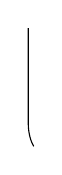
\begin{tikzpicture}[x=1cm,y=1cm]\draw (0,1.5)--(0,.3) .. controls (0,.15) and (.04,.05) .. (.07,0);\end{tikzpicture}}

En particulier, si $e=1$ cet hom. est l'identité, \deleted{\unsure{et}} et à fortiori un isomorphisme. \inserted{Ceci s'applique en particulier si $V'=\widetilde V$.} En fait, on a mieux.

\uline{Prop.} 3.13. Supposons $V'=\widehat V$, \deleted{et $V$ \unsure{excellent}} \inserted{\deleted{et $V$ excellent (i.e. $\widehat K$ sép. sur $K$).}} Alors les hom de suites exactes (3.5) et (3.7) sont des isomorphismes.

\deleted{
$\pi'\longrightarrow\pi$ \deleted{est \unsure{donc}} surjectif, i.e. si $K_1$ est une extension finie séparable de $K$, alors $K_1\otimes_K\widehat K$ est un corps. \deleted{et $I'_t\simeq I_t$} \inserted{La clôture \unsure{normale} $V_1$ de $V$ dans $K_1$ est \uline{\unsure{finie}} \unsure{sur $V$}, par suite $V_1\otimes_V\widehat V=\widehat V_1$ intègre (car $V_1$ est un anneau \inserted{de val. discrète); donc $K_1\otimes_K\widehat K=\widehat V_1\otimes_{\unsure{\widehat V}}\widehat K$ est un corps.}}
(Comme $\pi'_0\longrightarrow\pi_0$ est évidemment un isom., et aussi \inserted{$I'_t\mathrel{\text{---}}I_t$, par \unsure{l'injectivité|l'isomorphisme} de \unsure{$I'_t\mathrel{\text{---}}I_t$}}) on est ramené en fait à examiner $P'\mathrel{\text{---}}P$. Ceci \inserted{[ou directement $\pi'\longrightarrow\pi$, donc $I'\mathrel{\text{---}}I$)} est tjs injectif, d'après les résultats connus de \deleted{approximation} \inserted{continuité} des solutions d'une équation algébrique p. r. aux coefficients, qui \unsure{impliquent|expliquent} que des \unsure{équations|extensions} séparables \uline{voisines} définissent des extensions isomorphes de $\widehat K$. \deleted{D'autre part, c'est surjectif} \inserted{Comme $I'\longrightarrow I$ est surjectif} \inserted{(d'après les résultats} \deleted{\unsure{que donne précisément} l'hypothèse d'excellence}

\uline{Remarque} 3.14. La prop. 3.13. montre que dans la plupart des questions \deleted{\unsure{concernant}} du séminaire, on pourrait supposer $V$ \uline{complet}.
}
\margin{\deleted{\uline{Attention}}}
\margin{$\widetilde V\subset\widetilde{\widehat V}\subset\widehat{\widetilde V}$}
\margin{13}
